%%%%%%%%%%%%%%%%%%%%%%%%%%%%%%%%%%%%%%%%%%%%%
%% Capítulo 2 - Maximum Fragment Length
%% Copyright 2006 Eliézio Batista de Oliveira
%%%%%%%%%%%%%%%%%%%%%%%%%%%%%%%%%%%%%%%%%%%%%

\section{\acl{MFL}}

\subsection{Especificação}

\begin{lstlisting}[caption={RFC 3546, trecho da seção 3.2}]
The "extension_data" field of this extension SHALL contain: 
 
   enum{ 
       2^9(1), 2^10(2), 2^11(3), 2^12(4), (255) 
   } MaxFragmentLength; 
 
whose value is the desired maximum fragment length.  The allowed 
values for this field are: 2^9, 2^10, 2^11, and 2^12.
\end{lstlisting}

\subsection{Divergências}

O valor 5 ($2^{13}$ = 8192) é também aceito.

\subsection{API Estendida}

\begin{lstlisting}[language=C,%
		    emph={TLSX_CTX_set_maximum_fragment_length,TLSX_set_maximum_fragment_length},%
		    caption=API para a extensão \acs{MFL}]
/* ----- Client Side ----- */
void TLSX_CTX_set_maximum_fragment_length (
	SSL_CTX *ctx,
	int frag_length
);

void TLSX_set_maximum_fragment_length (
	SSL * ssl,
	int frag_length 
);
\end{lstlisting}

Em ambas as funções o valor efetivamente selecionado é menor tamanho válido 
segundo a especificação (512, 1024, 2048, 4096 ou 8192) que seja maior ou igual 
a \verb|frag_length|.

\subsection{Implementação}

\begin{description}[\breaklabel\setlabelstyle{\ttfamily}]

\item[s3\_srvr.c::ssl3\_get\_client\_hello]
	Modificada para efetivar o parâmetro \verb|tlsx_max_plain_length| em caso de 
	restauração de sessão. 

\item[s3\_clnt.c::ssl3\_get\_server\_hello]
	Após a restauração de uma sessão TLS (\emph{``session resumption''}), efetiva o 
	parâmetro \verb|tlsx_max_plain_length| imediatamente;

\end{description}

\subsection{Testes de Conformidade}

A validação da implementação dessa extensão é um pouco mais complexa, pois 
a ferramenta de captura e decodificação utilizada (\verb|tethereal|) não é capaz de 
tratar corretamente mensagens de \emph{handshake} desmembradas em mais de um 
registro TLS. Resta-nos, portanto, efetuar uma captura menos detalhada que 
explicite principalmente o tamanho de cada registro TLS e assim certificar-nos 
de que o tamanho de cada registro não excede ao \emph{maximum fragment length}
especificado, e se esta decomposição não interfere no perfeito fechamento do 
\emph{handshake}.

A captura diferenciada foi realizada usando-se a seguinte sintaxe na chamada 
do \verb|tethereal|:

\begin{lstlisting}[caption=Chamada do {\tt tethereal} para o detalhamento dos registros TLS]
tethereal -i eth0 \ 
-z "proto,colinfo,ssl.record.length,ssl.record.length" \ 
-z "proto,colinfo,tcp.len>0,tcp.len" \ 
port 443
\end{lstlisting}

O caso de teste escolhido consistiu em uma solicitação \acs{HTTPS} usando o método 
GET do arquivo \verb|README| da distribuição do OpenSSL que contém exatos 7930 
bytes. A chamada do \emph{script} \verb|s_client.sh| ficou, portanto:

\begin{lstlisting}[caption=Chamada do \texttt{s\_client.sh} para o teste da extensão \acs{MFL}]
./s_client.sh -tlsx_max_fragment_length 1024 -reconnect 1
\end{lstlisting}

\begin{lstlisting}[caption=Mensagem \tlsHsCh com a extensão \acs{MFL} habilitada]
Secure Socket Layer 
  SSL Record Layer: Handshake Protocol: Client Hello 
    Content Type: Handshake (22) 
    Version: TLS 1.0 (0x0301) 
    Length: 52 
    Handshake Protocol: Client Hello 
      Handshake Type: Client Hello (1) 
      Length: 48 
      Version: TLS 1.0 (0x0301) 
      Random.gmt_unix_time: Jan  6, 2006 11:27:27.000000000 
      Random.bytes 
      Session ID Length: 0 
      Cipher Suites Length: 2 
      Cipher Suites (1 suite) 
	Cipher Suite: TLS_RSA_WITH_RC4_128_SHA (0x0005) 
      Compression Methods Length: 1 
      Compression Methods (1 method) 
	Compression Method: null (0) 
      Extensions Length: 5 
      Extension: max_fragment_length 
	Type: max_fragment_length (|0x0001|) 
	Length: |1| 
	Data (1 byte) 

0000  00 c0 49 43 0b 55 00 50 04 aa 26 05 08 00 45 00   ..IC.U.P..&...E. 
0010  00 61 67 39 40 00 40 06 f4 1b 0a 04 02 14 c9 2d   .ag9@.@........- 
0020  09 fd e7 86 01 bb d6 f1 40 b0 30 5d 60 1a 50 18   ........@.0]`.P. 
0030  16 d0 54 f9 00 00 16 03 01 00 34 01 00 00 30 03   ..T.......4...0. 
0040  01 43 be 70 3f b9 60 f0 1c 02 1b 8f e7 35 db 4f   .C.p?.`......5.O 
0050  c8 da 03 81 fc 8e 66 fb 9a 9b f8 01 68 08 79 16   ......f.....h.y. 
0060  57 00 00 02 00 05 01 00 00 05 |00 01 00 01 02|      W.........|.....|
\end{lstlisting}

As duas conexões foram posteriormente analisadas e sintetizadas nas tabelas 
apresentas a seguir.

\subsubsection{Primeira conexão (\emph{full handshake})}

Pelo tráfego da primeira conexão, sintetizado na Tabela~\vref{tab:mfl_run1},
pode-se constatar a observância do limite imposto pelo \emph{maximum fragment length} 
pela presença dos diversos registros TLS para a composição da mensagem 
\tlsHsC enviada pelo servidor.

A Figura~\vref{fig:mfl_example} ilustra como a mensagem \tlsHsC é fragmentada em dois registros 
após a ativação dessa extensão, e como esses registros se distribuem entre dois segmentos TCP.


\begin{figure}[htb]
    \centering
        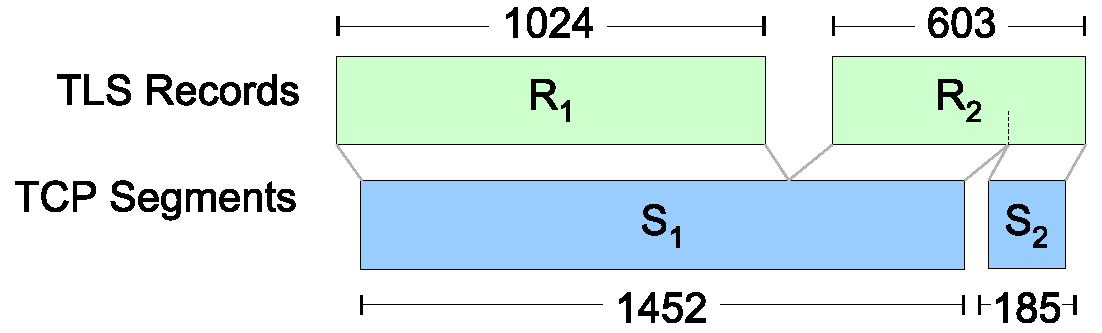
\includegraphics[scale=0.50]{fig/mfl_example}
    \caption{Fragmentação da mensagem \tlsHsC}
    \label{fig:mfl_example}
\end{figure}


\begin{table}[ht]
    \begin{center}
    \caption{\emph{Handshake} com registros limitados a 1024 bytes}
    \label{tab:mfl_run1}
	\begin{tabular}{@{}rclrl@{}} \toprule
%Time (s) & Direction & \multicolumn{2}{c}{TCP} & TLS Records [length] \\ \cmidrule(lr){3-4}
%         & C $\longleftrightarrow$ S &  Flags & Length & \\ \midrule
\tlsFlowHeader \\ \midrule
0.000000 & $\longrightarrow$ & SYN      &	& \\
\altrowcolor
0.028681 & $\longleftarrow$  & SYN, ACK &	& \\
0.028835 & $\longrightarrow$ & ACK      &	& \\
0.031536 & $\longrightarrow$ &		&    57 & Client Hello [52] \\
\altrowcolor
0.072442 & $\longleftarrow$  &		&    86 & Server Hello [81] \\
0.072600 & $\longrightarrow$ & ACK      &	& \\
\altrowcolor
0.096442 & $\longleftarrow$  &		&  1452 & Certificate R1 [1024], \\
\altrowcolor
	 &		     &	        &	& \hl{Certificate R2a} [418/603] \\
0.096567 & $\longrightarrow$ & ACK      &	& \\
\altrowcolor
0.096637 & $\longleftarrow$  &		&   185 & \hl{Certificate R2b} [185/603] \\
0.096708 & $\longrightarrow$ & ACK      &	& \\
\altrowcolor
0.143681 & $\longleftarrow$  &		&     9 & Server Hello Done [4] \\
0.143837 & $\longrightarrow$ & ACK      &	& \\
0.154354 & $\longrightarrow$ &		&   186 & Client Key Exchange [134], \\
	 &		     &		&	& Change Cipher Spec [1], \\
	 &		     &		&	& Finished [36] \\
\altrowcolor
0.328340 & $\longleftarrow$  & ACK      &	& \\
\altrowcolor
0.423803 & $\longleftarrow$  &		&     6 & Change Cipher Spec  [1] \\
0.466072 & $\longrightarrow$ & ACK      &	& \\
\altrowcolor
0.496468 & $\longleftarrow$  &		&    41 & Finished [36] \\
0.497304 & $\longrightarrow$ & ACK      &	& \\
0.500684 & $\longrightarrow$ &		&    27 & Alert - Close Notify [22] \\
0.500964 & $\longrightarrow$ & FIN, ACK &	& \\
\altrowcolor
0.532371 & $\longleftarrow$  & ACK      &	& \\
\altrowcolor
0.548267 & $\longleftarrow$  & FIN, ACK &	& \\
0.548366 & $\longrightarrow$ & ACK      &	& \\ \bottomrule
	\end{tabular}
    \end{center}
\end{table}

\subsubsection{Segunda conexão (\emph{resumed handshake})}

A segunda conexão realizada logo em seguida e cujos resultados estão sintetizados
na Tabela~\vref{tab:mfl_run2}, comprova duas outras 
funcionalidades:

\begin{enumerate}
\item Que após a restauração da sessão o limite do tamanho de cada registro 
voltou a ser o valor negociado na sessão anterior (1024); e
\item Esse limite é efetivo após o \emph{handshake}, como fica evidente pelo 
desmembramento da resposta (\emph{Application Data}) em 8 registros.
\end{enumerate}

\begin{table}[ht]
    \begin{center}
    \caption{Conexão TLS com registros limitados a 1024 bytes}
    \label{tab:mfl_run2}
	\begin{tabular}{@{}rclrl@{}} \toprule
%Time (s) & Direction & \multicolumn{2}{c}{TCP} & TLS Records [length] \\ \cmidrule(lr){3-4}
%         & C $\longleftrightarrow$ S &  Flags & Length & \\ \midrule
\tlsFlowHeader \\ \midrule
0.501275 & $\longrightarrow$ & SYN      &	& \\
\altrowcolor
0.533568 & $\longleftarrow$  & SYN, ACK &       & \\
0.533708 & $\longrightarrow$ & ACK      &       & \\
0.534627 & $\longrightarrow$ &          &    89 & Client Hello [84] \\
\altrowcolor
0.658061 & $\longleftarrow$  &          &    79 & Server Hello [74] \\
0.659113 & $\longrightarrow$ & ACK      &       & \\
\altrowcolor
0.691062 & $\longleftarrow$  &          &    47 & Change Cipher Spec [1], \\
\altrowcolor
         &                   &          &       & Finished [36] \\
0.696049 & $\longrightarrow$ & ACK      &       & \\
0.697457 & $\longrightarrow$ &          &    47 & Change Cipher Spec [1], \\
         &                   &          &       & Finished [36] \\
\altrowcolor
0.926678 & $\longleftarrow$  & ACK      &       & \\
8.144505 & $\longrightarrow$ &          &    46 & Application Data [41] \\
\altrowcolor
8.260117 & $\longleftarrow$  &          &  1049 & Application Data R1 [1044] \\
\altrowcolor
8.286967 & $\longleftarrow$  &          &  1452 & Application Data R2 [1044], \\
\altrowcolor
         &                   &          &       & \hl{Application Data R3a} [398/1044] \\
8.287067 & $\longrightarrow$ & ACK      &       & \\
\altrowcolor
8.291990 & $\longleftarrow$  &          &   646 & \hl{Application Data R3b} [646/1044] \\
\altrowcolor
8.308943 & $\longleftarrow$  &          &  1452 & Application Data R4 [1044], \\
         &                   &          &       & \hl{Application Data R5a} [398/1044] \\
8.309037 & $\longrightarrow$ & ACK      &       & \\
\altrowcolor
8.314126 & $\longleftarrow$  &          &   646 & \hl{Application Data R5b} [646/1044] \\
\altrowcolor
8.338292 & $\longleftarrow$  &          &  1452 & Application Data R6 [1044], \\
\altrowcolor
         &                   &          &       & \hl{Application Data R7a} [398/1044] \\
8.338386 & $\longrightarrow$ & ACK      &       & \\
\altrowcolor
8.343465 & $\longleftarrow$  &          &   646 & \hl{Application Data R7b} [646/1044] \\
\altrowcolor
8.377197 & $\longleftarrow$  &          &   832 & Application Data R8 [827] \\
8.377291 & $\longrightarrow$ & ACK      &       & \\
8.379235 & $\longrightarrow$ &          &    27 & Alert - Close Notify [22] \\
8.379346 & $\longrightarrow$ & FIN, ACK &       & \\
\altrowcolor
8.456271 & $\longleftarrow$  & ACK      &       & \\ \bottomrule
	\end{tabular}
    \end{center}
\end{table}

